\documentclass[a4paper,12pt, twoside]{article}
%\documentclass[a4paper,12pt, twoside]{book}

\usepackage[papersize={210mm,297mm},tmargin=20mm,bmargin=20mm,lmargin=20mm,rmargin=20mm]{geometry}

\usepackage[utf8]{inputenc}
%https://mirror.hmc.edu/ctan/macros/latex/contrib/babel-contrib/turkish/turkish.pdf
\usepackage[english]{babel}
%\usepackage[T1]{fontenc}

\usepackage{amsmath,amssymb,mathabx}%\for eqref
\usepackage{lscape}

\usepackage{hyperref}
\hypersetup{
    colorlinks,
    citecolor=black,
    filecolor=black,
    linkcolor=blue,
    urlcolor=red}
  

%%% \usepackage{svg}
%%% https://tex.stackexchange.com/questions/122871/include-svg-images-with-the-svg-package/129854
\usepackage{graphicx}
\graphicspath{ {./figurler/} }

\usepackage[colorinlistoftodos]{todonotes}
\usepackage{fancyhdr}

\usepackage{indentfirst}
%% paragraf girintisi
\setlength{\parindent}{5ex}

%% Daha sonra yazılacak kısımları not düşmek için...
\newcommand{\YAZILACAK}{{\vspace{18pt}\bf\Large \color{red} YAZILACAK}}


\pagestyle{fancy}
\fancyhf{}
\lhead{ Kuantum Fiziği }
\chead{\thepage}
\rhead{Mesut Karakoç}
\lfoot{Akdeniz Üniversitesi}
\cfoot{}
%\rfoot{BF}

\title{Akdeniz Üniversitesi\\ Fen Fakültesi - Fizik Bölümü\\FİZ319 Kuantum Fiziği Ders Notları}

\author{\setlength{\unitlength}{6mm}
\begin{picture}(10,10)
\put(1.1,0){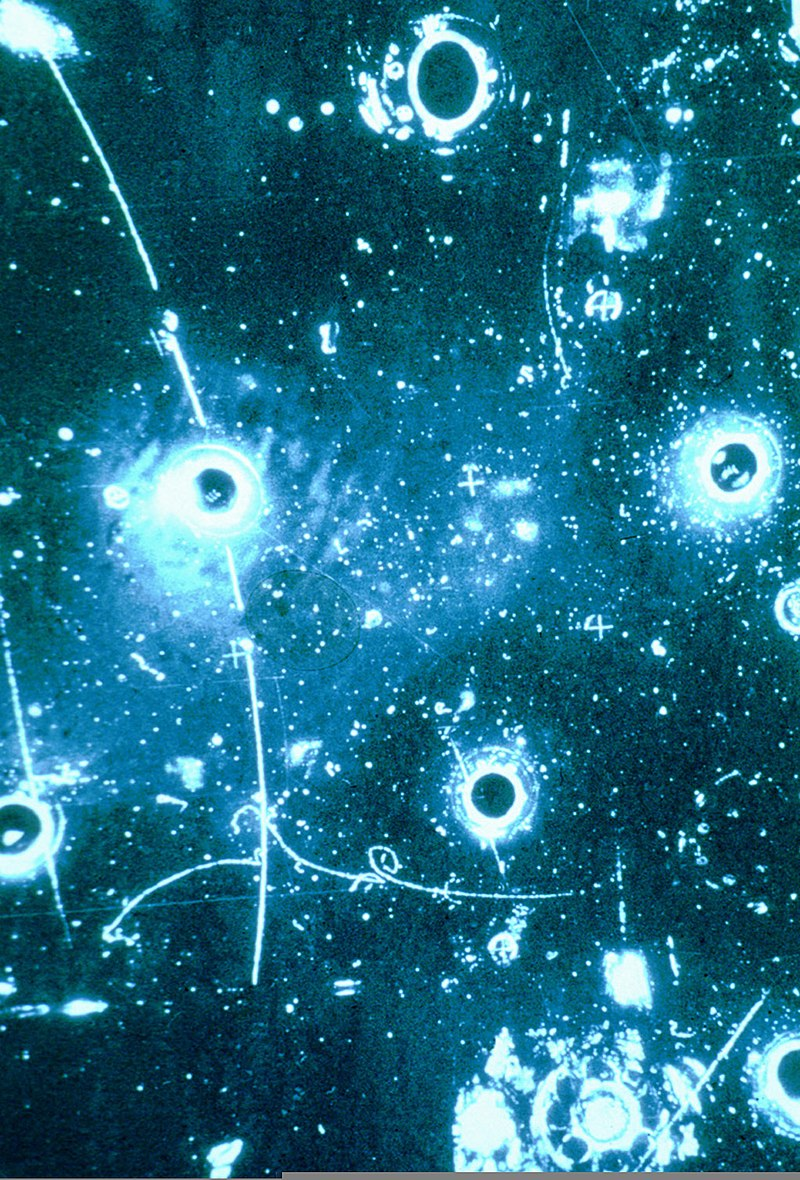
\includegraphics[width=4.5cm]{Leptonic_event_in_Gargamelle_bubble_chamber.jpg}}
\end{picture} \\ Doç. Dr. Mesut Karakoç}


\date{\today}

\begin{document}

%% Turkish babel problem
%% https://tex.stackexchange.com/questions/160385/newgeometry-doesnt-work-with-turkish-babel-package
%%\shorthandoff{=}% Make = not active any more

\maketitle

\newpage

% change name to "İçindekiler"
\renewcommand{\contentsname}{İçindekiler}
\tableofcontents{}

\listoffigures
 
\listoftables

\newpage

{
\hspace{.5\textwidth}
\begin{minipage}{.5\textwidth}
\raggedleft
If all this damned quantum jumps were really to stay, I should be
sorry I ever got involved with quantum theory.

—Erwin Schrödinger
\cite{book:Ficek}

%% Latince için
%% post iacturam quis non sapit!
%% Who is not wise after he has lost something?
%% https://quizlet.com/23756827/latin-proverbs-h-flash-cards/
\end{minipage}
}

\setcounter{section}{3} %% THIS WILL BE DELETED when all chapters merged!
\section{Bir Boyutlu Potansiyeller}

Üç boyutlu bir evrende yaşıyor olmamıza rağmen, bir çok fiziksel olayı (hareketi) bir boyutlu olarak tanımlamak mümkündür. Bu nedenle bu bölümde klasik fiziğin açıklayamadığı fakat kuantum fiziğiyle çalışabildiğimiz bazı bir boyutlu sistemleri inceleyeceğiz.


\subsection{Basamak Potansiyeli}
%%
\begin{figure}[hbtp]
	\centering
	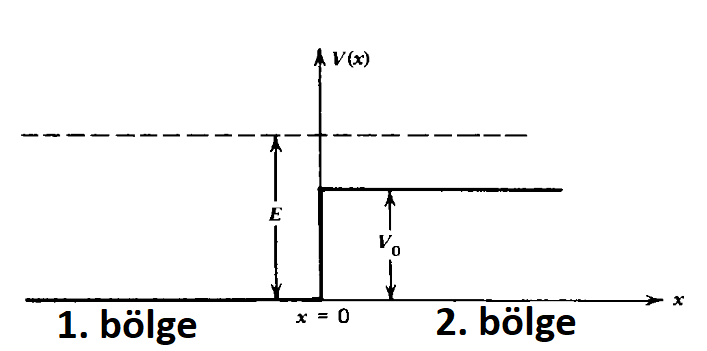
\includegraphics[width=0.7\linewidth]{figurler/Basamak_Potansiyeli}
	\caption{Basamak potansiyeli.}
	\label{fig:basamakpotansiyeli}
\end{figure}
%%
Basamak potansiyeli için bir örnek yukarıdaki şekildeki gibi olur. Şekilden anlaşılacağı üzere basamak potansiyeli; birbirinden farklı sabit potansiyellere sahip iki bölge içeren bir durumdur. Bir boyutlu hali için matematiksel ifadesi aşağıdaki gibidir.
%%
\begin{equation}
V ( x )  = \left\{ 
\begin{array} { l l } 
{ 0 } & {\Leftarrow x < 0 } \\ 
{ V _ { 0 } } & {\Leftarrow x \geq 0 } 
\end{array} \right. 
\end{equation}
%%

Bu potansiyeli zamandan bağımsız Schrödinger denklemi ile çalışabiliriz. Öncelikle Schrödinger denklemini yazılışı daha kolay olan,
%%
\begin{equation}
- \frac { \hbar ^ { 2 } } { 2 m } \frac { d ^ { 2 } u ( x ) } { d x ^ { 2 } } + V ( x ) u ( x ) = E u ( x )
\end{equation}
%%
formuna dönüştürebiliriz.

\begin{equation}
\frac { d ^ { 2 } u ( x ) } { d x ^ { 2 } } + \frac { 2 m } { \hbar ^ { 2 } } [ E - V ( x ) ] u ( x ) = 0
\end{equation}
%%
Basamak potansiyelinin değerinin sıfır olduğu bölge için,
%%
\begin{equation}
\frac { 2 m} { \hbar ^ { 2 } } E = k ^ { 2 }
\end{equation}
%%
tanımını ve sıfırdan farklı olduğu bölge için
%%
\begin{equation}
\frac { 2 m} { \hbar ^ { 2 } }  \left( E - V _ { 0 } \right) = q ^ { 2 }
\end{equation}
%%
tanımını yapabiliriz. $x<0$ ve $V(x)=0$ bölgesi için çözüm
%%
\begin{equation}
u_1 ( x ) \equiv u ( x ) = A e ^ { i k x } + B e ^ { - i k x }
\end{equation}
%%
olarak yazılabilir. Burada $A e ^ { i k x }$, $x=-\infty$'deki bir kaynaktan gelen serbest düzlem dalga olarak düşünülebilir, $B e ^ { -i k x }$ ise $x=0$ noktasında ortam değişikliğinden dolayı yansıyan dalga olarak düşünülebilir. Bu bölgedeki toplam olasılık akısı,
%%
\begin{equation}
\begin{array} { r l } 
{ j_1 } &\equiv  j  = \frac { \hbar } { 2 i m } \left( u ^ { * } \frac { d u } { d x } - \frac { d u ^ { * } } { d x } u \right) \\
& = \frac { \hbar } { 2 i m } \left[ \left(A^{*} e ^ { - i k x } + B ^ { * } e ^ { i k x } \right) \left(i k A e ^ { i k x } - i k B e ^ { - i k } \right) - \left( -i k A^{*} e ^ { -i k x } + i k B^* e ^ {  i k } \right) \left( A e ^ { i k x } + B  e ^ { -i k x } \right)  \right]  \\ 
{ } & { = \frac { \hbar k } { m } \left( | A | ^ { 2 }  - | B | ^ { 2 } \right) } \end{array}
\end{equation}
%%
olur. $x>0$ ve $V(x)=V_0$ için ise,
%%
\begin{equation}
u_2 ( x ) \equiv u ( x ) =  C e ^ { i q x }
\end{equation}
%%
çözümü elde edilir. Sadece $C e ^ { i q x }$ kısmı vardır, çünkü bu bölge $x=+\infty$'a kadar uzanmaktadır ve potansiyel sabittir bu yüzden, yansıyan dalga söz konusu değildir. Sadece $+x$ yönünde ilerleyen olasılık dalgası vardır. Bu olasılık dalgası için olasılık akısı,
%%
\begin{equation}
j_2 \equiv j = \frac { \hbar q } { m } | C | ^ { 2 }
\end{equation}
%%
bulunur. Her iki bölgedeki olasılık akıları ($j_1 = j_2$) birbirine eşit olmalıdır. Eğer,
%%
\begin{equation}
\frac { \partial } { \partial t } P ( x , t ) + \frac { \partial } { \partial x } j ( x , t ) = 0
\end{equation}
%%
olduğu hatırlanırsa ve kısmi değişkenlere ayrılabilir dalga fonksiyonu ile çalıştığımızdan $P(x, t) = \psi(x,t) \psi^*(x,t) = u(x) u^*(x)$ olacağına göre,
%%
\begin{equation}\label{key}
\frac { \partial } { \partial t } P ( x , t ) = \frac { \partial } { \partial t } |u ( x)|^2 = 0
\end{equation}
%%
elde edilir. Buradan,
%%
\begin{equation}
\frac { \partial } { \partial x } j ( x , t ) = 0
\end{equation}
%%
sonucuna ulaşırız. $x=0$ civarında $x=\pm\varepsilon \rightarrow 0$ aralığında yukarıdaki ifadenin integrali,
%%
\begin{equation}
\int^{\varepsilon}_{-\varepsilon} dx \frac { \partial } { \partial x } j ( x , t ) = j (\varepsilon  , t ) - j ( -\varepsilon , t ) = 0
\end{equation}
%%
sonucunu verir. Böylece $j_1 = j_2$ olması gerektiği ortaya çıkar. Her iki bölgedeki olasılık akıları da $x$'ten bağımsız olduklarından sınırda eşitlerse bütün tanımlı uzay boyunca birbirlerine eşit olmalıdırlar,
%%
\begin{equation}
\frac { \hbar k } { m } \left( | A | ^ { 2 }  - | B | ^ { 2 } \right) = \frac { \hbar q } { m } | C | ^ { 2 }
\end{equation}
%%
yukarıdaki eşitlikle bu sonuç ifade edilmiş olur. Dalga fonksiyonlarının $x=0$'daki sürekliliğinden ise,
%%
\begin{align}
u_1(0) &= u_2(0) \\
A + B  &= C
\end{align}
%%
elde edilir. Basamak potansiyeli $x=0$'da süreksiz olmasına rağmen, sistemin dalga fonksiyonu $u(x)$ süreklidir, dalga fonksiyonun türevinin de $x=0$'da sürekli olacağı aşağıda verilen matematik süreçle gösterilmiş olur.
%%
\begin{equation}
\begin{array} { r l } { \left( \frac { d u } { d x } \right) _ { +\varepsilon } - \left( \frac { d u } { d x } \right) _ { - \varepsilon } } & { = \int _ { - \varepsilon } ^ { +\varepsilon } d x \frac { d } { d x } \frac { d u } { d x } } \\ { } & { = \int _ { - \varepsilon } ^ { +\varepsilon } d x \frac { 2 m } { \hbar ^ { 2 } } [ V ( x ) - E ] u ( x ) = 0 } \end{array}
\end{equation}
%%
Burada $\varepsilon$ sonsuz küçük bir pozitif reel sayıdır. $x=0$'ın $-\varepsilon$ ve $+\varepsilon$ civarında dalga fonksiyonlarının türevlerinin farkı yukarıdaki eşitliğin sol tarafındaki gibidir ve bu farkın integral formuda eşitliğin sağ tarafındaki gibidir. Eşitliğin sol tarafı Schrödinger denkleminden faydalanılarak $V(X)$, $E$ ve $u(x)$'i içerecek şekilde yeniden yazılabilir. Bu problemde $V(x)$ ve $E$ birer sabit sayı olduklarından, $\pm \varepsilon \rightarrow \infty$ olduğundan ve böylece $u(x)$'in sürekliliği gerçekleştiğinden bu integralin cevabı sıfır olacaktır. Böylece bu tür problemler için dalga fonksiyonlarının türevlerinin de  sürekli oldukları kabul edilebilir. 

Yeri geldiğinden ve daha sonra kullanılacağı için şimdiden belirtmek gerekir ki, bu süreklilik $\lambda \delta(x-a)$ benzeri Dirac-delta fonksiyonu içeren potansiyeller için geçerli değildir. Böyle potansiyeller için süreklilik aşağıdaki gibi bir süreksizlik halin alır.
%%
\begin{equation}
\begin{aligned} \left( \frac { d u } { d x } \right) _ { a + \varepsilon } - \left( \frac { d u } { d x } \right) _ { a - \varepsilon } & = \frac { 2 m } { \hbar ^ { 2 } } \int _ { a - \varepsilon } ^ { a + \varepsilon } d x \lambda \delta ( x - a ) u ( x ) \\ & = \frac { 2 m } { \hbar ^ { 2 } } \lambda u ( a ) \end{aligned}
\end{equation}
%%

Bu problemde türevlerinin sürekliliği sağlandığına göre; türevlerinin sürekliliğinden,
%%
\begin{align}
\frac{d}{dx}u_1(x) \bigg|_{x=0-} &= \frac{d}{dx}u_2(x) \bigg|_{x=0+} \\
i k ( A - B ) &= i q C
\end{align}
%%
elde edilir.

Bu tür problemleri çalışılırken, klasik bir dalga sisteminin davranışına benzer olarak yansıma ve geçme olasılıklarından bahsetmek mümkündür. Bu olasılıklarla ilişklili olarak, genellikle yansıma ve geçme katsayıları, sırasıyla,
%%
%%
\begin{align}
R \equiv \frac{|j_\text{yansıyan}|}{|j_\text{gelen}|} \\
T \equiv \frac{|j_\text{geçen}|}{|j_\text{gelen}|}
\end{align}
%%
şeklinde tanımlanırlar. $R$ ve $T$'yi hesaplamadan önce olasılık akısı üzerinde biraz daha bilgilerimizi genişletmeliyiz: olasılık akısını üç boyutlu durum için yazacak olursak,
%%
\begin{equation}
\vec j = \frac{\hbar}{2 m i} \left[
\Psi^*(\vec r, t) \vec \nabla \Psi(\vec r, t) - 
\Psi(\vec r, t) \vec \nabla \Psi^*(\vec r, t)
\right]
\end{equation}
%%
bir vektör davranışına sahip olduğu açıkca görülür. Basamak potansiyeli probleminde, $j_1$ aslında,
%%
\begin{equation}
\vec j_1 = \vec j_\text{gelen} + \vec j_\text{yansıyan}
\end{equation}
%%
olarak yazılabilir. $j_2$ ise,
%%
\begin{equation}
\vec j_2 = \vec j_\text{geçen}
\end{equation}
%%
olarak yazılabilir. Akının korunumu ise,
%%
%%
\begin{equation}
\vec j_\text{gelen} + \vec j_\text{yansıyan} = \vec j_\text{geçen}
\end{equation}
%%
olmasını gerektirir. Tekrar basamak potansiyeli çalıştığımız bir boyutlu duruma döner ve vektör notasyonunu bırakırsak ve yönleri sadece $+$ ve $-$ işaretleriyle temsil edersek,
%%
\begin{equation}
j_\text{gelen} =  \frac{\hbar}{2 m i} \left[u^*_g \frac{d}{dx}u_g - u_g (\frac{d}{dx}u_g)^*\right]
\end{equation}
%%
olur. Burada $u_g = A e ^ { i k x } $ ile verilir ve $x=-\infty$'den gelen dalga fonksiyonunu temsil eder. Böylece gelen akı,
%%
\begin{equation}
j_\text{gelen} =  \frac{\hbar k}{m} |A|^2
\end{equation}
%%
olur. Benzer şekilde, yansıyan dalga $u_y = B e ^ { -i k x } $ ve geçen dalga $u_t = C e ^ { i q x } $ ifadeleri ile tanımlanırlar. Böylece yansıyan ve geçen olasılık akıları,
%%
\begin{equation}
j_\text{yansıyan} =  -\frac{\hbar k}{m} |B|^2 \quad \text{ ve } \quad
j_\text{geçen} =  \frac{\hbar q}{m} |C|^2 
\end{equation}
%%
olarak bulunurlar. Yansıma ve geçme katsayıları ise,
%%
%%
\begin{equation}
R =  \frac{|B|^2}{|A|^2} \quad \text{ ve } \quad
T =  \frac{q}{k} \frac{|C|^2}{|A|^2}
\end{equation}
%%
olarak bulunurlar. $R$ ve $T$'yi bilinmeyen $A$, $B$ ve $C$ kat sayılarından
kurtarabiliriz. Bunun için akının korunumundan, dalga fonksiyonlarının ve türevlerinin sürekliliğinden,
%%
%%
\begin{align}
\frac { \hbar k } { m } \left( | A | ^ { 2 }  - | B | ^ { 2 } \right) &= \frac { \hbar q } { m } | C | ^ { 2 }\\
A + B  &= C \\
i k ( A - B ) &= i q C
\end{align}
%%
elde ettiğimiz yukarıdaki eşitlikleri kullanabiliriz. Olasılık akısının korunumundan elde ettiğimiz denklemin yardımıyla, kolayca,
%%
\begin{equation}
T + R =  \frac{q}{k} \frac{|C|^2}{|A|^2} + \frac{|B|^2}{|A|^2} = 1
\end{equation}
%%
olacağı gösterilebilir. Sürekliliklerden elde edilen denklemlerden de,
%%
\begin{equation}
B =  \frac{k-q}{k+q} A \quad \text{ ve } \quad
C =  \frac{2k}{k+q} A
\end{equation}
%%
olacağı gösterilebilir. Böylece $R$ ve $T$,
%%
\begin{equation}
R =  \left(\frac{k-q}{k+q}\right)^2  \quad \text{ ve } \quad
T =  \frac{4kq}{(k+q)^2}
\end{equation}
%%
olarak bulunurlar. 

$E<V_0$ durumu için dalga fonksiyonu,
%%
\begin{equation}
u ( x ) = T e ^ { - \eta x }
\end{equation}
%%
halini alır. Burada $\eta$ ($V_0>E$ olduğundan),
%%
\begin{equation}
\frac { 2 m} { \hbar ^ { 2 } }  \left(V _ { 0 } -E \right) = \eta ^ { 2 }
\end{equation}
%%
olarak tanımlanır. Benzer bir matematiksel süreçten geçilerek hesaplar yapıldığında dalga fonksiyonu genlikleri arasınada,
%%
\begin{equation}
B =  \frac{ik + \eta}{i k- \eta} A \quad \text{ ve } \quad
C =  \frac{i 2k}{i k-\eta} A
\end{equation}
%%
ilişkileri bulunur. Olasılık akıları hesaplandında, gelen ve yansıyan akıların aynı kaldığı, fakat geçen akının sıfır olduğu görülecektir. Bu nedenle her ne kadar basamağın içine giren dalga fonksiyonunun genliği $C$ sıfır olmasa da $j_\text{geçen} = 0$ olduğundan, geçme olasılığı katsayısı,
\begin{equation}
T = \frac{|j_\text{geçen}|}{|j_\text{gelen}|} = 0
\end{equation}
%%
olur. Yansıma olasılığı katsayısı ise,
%%
\begin{equation}
R = \frac{B B^*}{A A^*} = \left(  \frac{ik + \eta}{i k- \eta} \right) \left( \frac{ik - \eta}{i k + \eta} \right)  = 1
\end{equation}
%%
olur. Aşağıdaki şekillerde $R$, $T$ ve dalga fonksiyonlarının genliklerinin $E/V_0$ oranına göre davranışları gösterilmiştir.

\begin{figure}[!hbtp]
	\begin{minipage}{.5\textwidth}
		\centering
		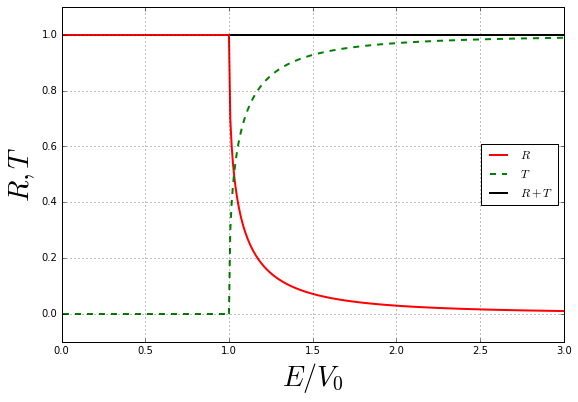
\includegraphics[width=1.0\linewidth]{Basamak_Potansiyeli_TR_EV0_grafigi.png}
		\caption{Yansıma ve geçiş katsayılarının $E/V_0$'a göre davranışları.}
		\label{fig:basamakpotansiyelitrev0grafigi}
	\end{minipage}
	\begin{minipage}{.5\textwidth}
		\centering
		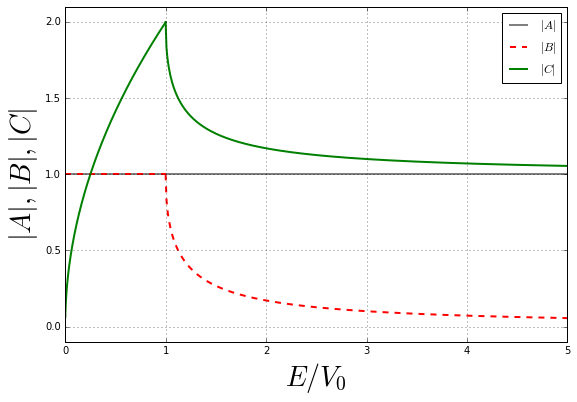
\includegraphics[width=1.0\linewidth]{Basamak_Potansiyeli_ABC_EV0_grafigi.png}
		\caption{Dalga fonksiyonu genliklerinin $E/V_0$'a göre davranışları.}
		\label{fig:basamakpotansiyeliABCev0grafigi}
	\end{minipage}
\end{figure}

Elde edilen sonuçlar hakkında bazı fiziksel yorumlar yapılabilir:
\begin{itemize}
	\item Klasik mekanik açısından bakıldığında buradaki yansıma olayı ilginçtir. Çünkü, bir potansiyelden geçen bir parçacığın kinetik enerjisini kaybedip, potansiyel enerjiye dönüştürerek, yavaşlaması beklenir. Burada gözlediğimiz yansıma davranışı ancak ilgilendiğimiz sistemdeki parçacıkların dalga davranışı gösterdiklerini ve dalga mekaniği davranışına uygun davrandıklarını göstermektedir.
	
	\item $T + R = 1$ olması olasılık akısının korunumunun geçerliliğini onaylamaktadır. Eğer bütün parçacıkların, bütün uzay içerisinde var olma olasılığı $1$ ise yansıma ve geçme olasılıklarının toplamının $1$ olması, korunumun sağlandığını göstermektedir.
	
	\item $E>>V_0$ için $R\rightarrow0$ ve $q\rightarrow k$, bunun nedeni kolayca anlaşılabilir. Parçacığın veya sistemin enerjisi arttıkça basamak potansiyelinin etkisi neredeyse yok gibidir.
	
	\item $E<V_0$ ise
	
\end{itemize}

\subsection{Sonlu Potansiyel Kuyusu}

\newpage
% In the preamble, add "\renewcommand\refname{New Title}" for article type documents 
% and "\renewcommand\bibname{New Title}" for book and report type documents.
\renewcommand\refname{Kaynaklar}
\bibliography{quantumBIB}{}
%% https://www.sharelatex.com/learn/latex/bibtex_bibliography_styles
 \bibliographystyle{plain}
%% \bibliographystyle{alpha}
%%\bibliographystyle{apalike}
\end{document}

